\subsection{Mínimo y máximo de funciones convexas}
~\medskip

En esta parte se considerarán problemas de minimizar y maximizar una función convexa sobre un conjunto convexo y se desarrollaran las 
condiciones necesarias y suficientes para optimalidad \cite{no-lineal}.\\ 
\medskip
\

{\definicion Sea $f: \mathbb{R}^n \longmapsto \mathbb{R}$ y consideremos el problema a minimizar $f(x)$ sujeto a $x \in S.$ Un punto $x \in S$ 
es llamado \textbf{\itshape solución factible} para el problema. Si $\overline{x} \in S $ y $ f(x) \geqslant f(\overline{x})$ para cada $x \in 
S,\,\, \overline{x} $ es llamado una \textbf{\itshape solución optima, solución optima global} o simplemente una \textbf{\itshape solución}
para el problema. \label{sol-problem}  }\\

La colección de soluciones óptimas es llamada \textbf{\itshape solución óptima alternativa.} 
\begin{itemize}
   \item Si $\overline{x} \in S$ y si existe un $\varepsilon-$vecindario $N_{\varepsilon}(\overline{x})$ alrededor de $\overline{x}$ tal que $ f(x) \geqslant f(\overline{x})$ para
	 cada $x \in S \cap N_{\varepsilon}(\overline{x}), \,\, \overline{x} $ es llamado \textbf{\itshape solución óptima local.}
   \item Si $\overline{x} \in S$ si $ f(x) > f(\overline{x})$ para todo $ x \in S \cap N_{\varepsilon}(\overline{x}), \,\,
	 x \neq \overline{x}$ para algún $\varepsilon > 0,\,\, \overline{x} $ es llamada \textbf{\itshape solución óptima local estricta}.
   \item Si $\overline{x} \in S$ es el único mínimo local en $ S \cap N_{\varepsilon}(\overline{x}), $ para algún vecindario
	 $N_{\varepsilon}(\overline{x})$ alrededor de $\overline{x}, \,\, x\,$ es llamada \textbf{\itshape solución óptima local fuerte o 
	 aislada}
\end{itemize}
~\medskip

Todos estos tipos de \'optimo local o m\'inimo local a veces tambi\'en se denominan como \textbf{\itshape m\'inimo relativo.} La 
Figura(\ref{mins}) ilustra ejemplos de m\'inimos locales y globales para el problema de minimizar $f(x)$ sujeto a $x \in S$

\begin{figure}
   \centering
   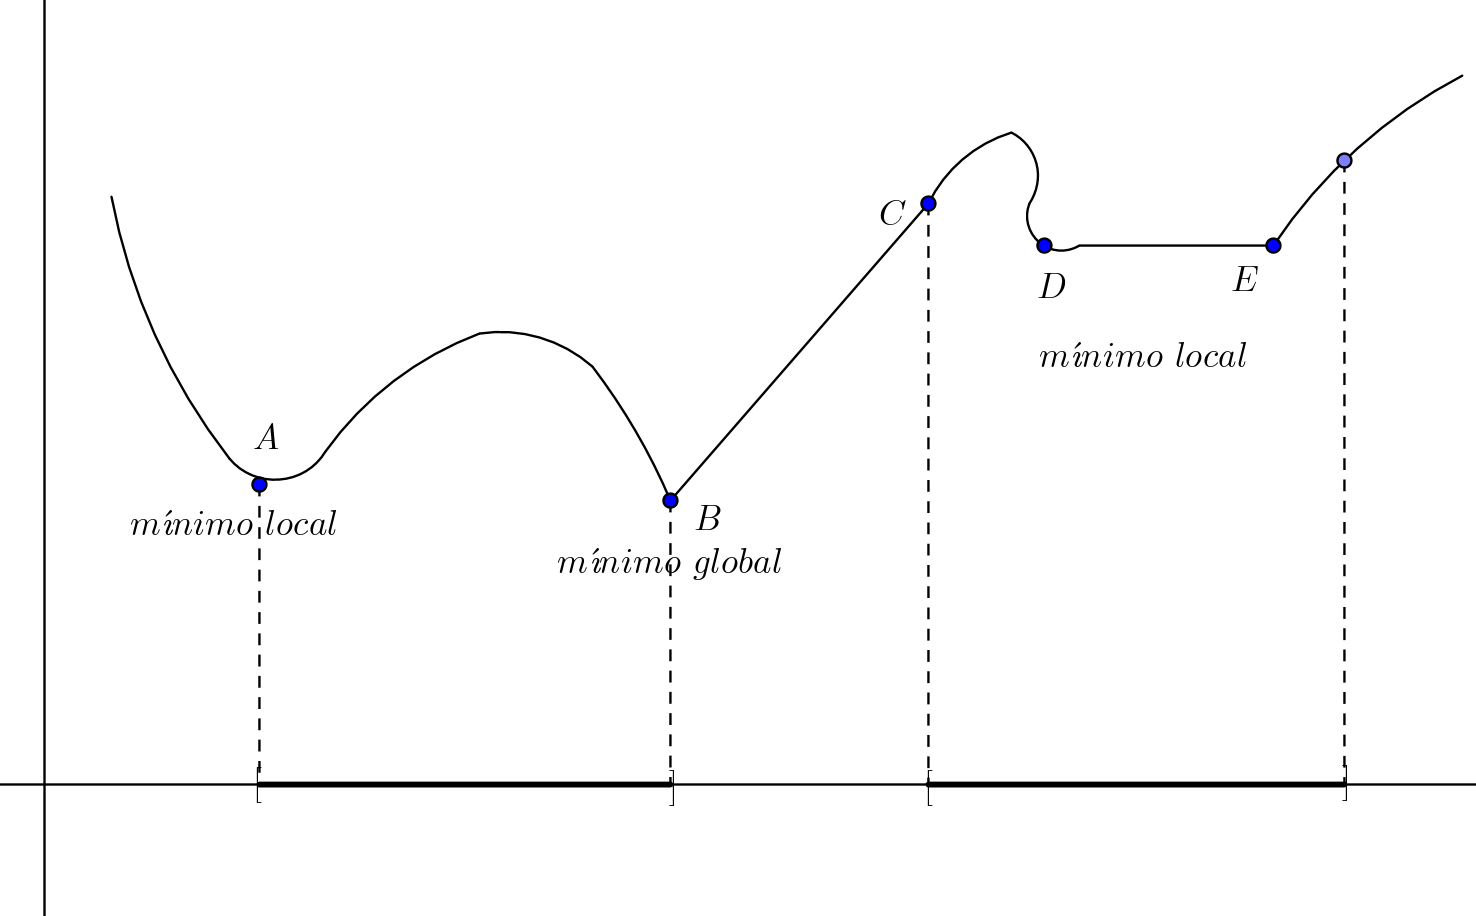
\includegraphics{./partes/sub_sec/codigo-image/minimos.png}
   \caption{M\'inimo local y global \cite{no-lineal}}
   \label{mins}
\end{figure}
\medskip

{\teorema Sea $S$ un conjunto convexo no vac\'io en $\mathbb{R}^n$ y sea $f: S \longmapsto \mathbb{R}$ convexa en $S.$ Considere minimizar el
problema $f(x)$ sujeto a $x \in S.$ Suponga que $\overline{x} \in S$ es una soluci\'on \'optima local para el problema, entonces:
\begin{enumerate}
   \item $\overline{x}$ es una soluci\'on \'optima global.
   \item Si $\overline{x}$ es una soluci\'on m\'inima estricta o $f$ es estrictamente convexa, $\overline{x}$ es la \'unica soluci\'on 
	 \'optima global y tambi\'en es un m\'inimo local.
\end{enumerate} \label{teo1-sol}}
~ \medskip

Acontinuaci\'on, se presenta una condici\'on necesaria y suficiente para la existencia de una soluci\'on global. Si tal soluci\'on \'optima no
existe, entonces $\inf \{f(x): x \in S \}$ es finito, pero no se alcanza en ning\'un punto de $S$ \'o es igual a $- \infty.$

{\teorema Sea $f$ una funci\'on convexa en $\mathbb{R}^n$ y $S$ un conjunto convexo en $\mathbb{R}^n$ Consideremos el problema de 
optimizaci\'on
\[\displaystyle{\min_{_{x \in S}} f(x)}\]

Entonces $\overline{x}$ es un m\'inimo local de $f$ sobre $S$ si y s\'olo si existe $s \in \partial f(\overline{x})$ tal que
\[\langle s, x - \overline{x} \rangle \geqslant 0 \,\, \mbox{ para toda } \, x \in S\]  \label{teo-important}}
\medskip

\textbf{Maximizar una funci\'on convexa}\\
\

Se desarrollar\'a una condici\'on necesaria para un m\'aximo de una funci\'on convexa sobre un conjunto convexo. Desafortunadamene, esta
condici\'on no es suficiente. Por lo tanto, es improbable, que varios m\'aximos que satisfagan la condici\'on del Teorema \ref{teo-max} 
existan. En el caso de mimizar, no existe informaci\'on local de tales soluciones que podr\'ian llevar a mejores puntos. Por lo tanto, 
maximizar una funci\'on convexa es una tarea mucho m\'as dura que minimizar una funci\'on convexa.\\ \\

{\teorema Sea $f: \mathbb{R}^n \longmapsto \mathbb{R}$ una funci\'on convexa y sea $S$ un conjunto convexo no vac\'io en $\mathbb{R}^n.$
Considere el problema:
\[\max_{{x \in S}} f(x)\]
Si $\overline{x} \in S$ es una soluci\'on \'optima local 
\[\langle s, x - \overline{x} \rangle \leqslant 0\]

para cada $x \in S$, donde $s \in \partial f(\overline{x})$ \label{teo-max}}




